\documentclass[9pt]{beamer}
\usepackage{styles/mypreamble}
%~~~~~~~~~~~~~~~~~~~~~~~~~~~~~~~~~~~~~~~~~~~~~~~~~~~~~~~~~~~~~~~~~~~~~~~~~~~~~~
\title{Алгоритмы машинного обучения}
\subtitle{Лекция 4. Методы понижения размерности}
\author{Владимир Кукушкин}
\institute{СПбГЭУ - 02.12.2020}
%~~~~~~~~~~~~~~~~~~~~~~~~~~~~~~~~~~~~~~~~~~~~~~~~~~~~~~~~~~~~~~~~~~~~~~~~~~~~~~

\begin{document}

\titlepage

\section{Постановка задачи}

\begin{frame}{Постановка задачи}
\begin{itemize}
    \item $p$-мерное пространство слишком сложно для восприятия.
    \item Хочется спроецировать точки из исходного $p$-мерного пространства на гиперплоскость привычной размерности.
    \item Тогда можно будет визуализировать все кластеры.
    \item Но в некоторых областях применения особенно ценится сжатие данных.
\end{itemize}
\end{frame}

\section{Метод главных компонент (PCA)}
\begin{frame}{Идея алгоритма}
\begin{itemize}
    \item Что значит информативность фичи? 
    \item Информативность можно ассоциировать с дисперсией. Фичи с константными значениями можно выбрасывать сразу же.
    \item Хотим спроецировать данные в такое подпространство, чтобы дисперсия вдоль его базиса была максимальной.
    \item Размерность подпространства можем выбирать самостоятельно.
    \item Проецирование -- линейное преобразование.
\end{itemize}
\begin{center}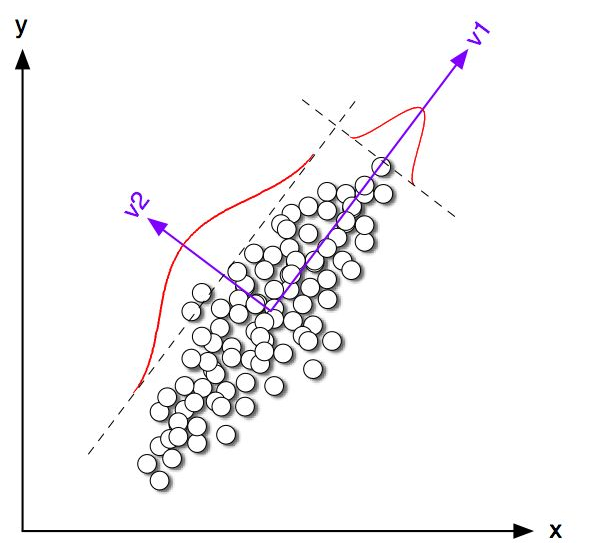
\includegraphics[width=150px]{img/pca_idea.png}\end{center}
\end{frame}

\begin{frame}{Формализация задачи}
\begin{itemize}
    \item Хотим найти такое преобразование $f(\lambda)=\mu + \textbf{V}_q\lambda$, $f: \mathbb{R}^q \rightarrow \mathbb{R}^p$, чтобы минимизировать функционал:
    \begin{equation}\label{pca_min}\min_{\mu, \{\lambda i\}, \textbf{V}_q} \sum_{i=1}^N \|x_i - (\mu + \textbf{V}_q\lambda)\|^2.\end{equation}
    \item Из курса линейной алгебры известно т.н. SVD-разложение матрицы (singular value decomposition):
    $$\textbf{X} = \textbf{U}\textbf{D}\textbf{V}^T,$$
    где $\textbf{U}, \textbf{V}$ -- ортогональные ($\textbf{U}^T\textbf{U}=\textbf{I}_p$), $\textbf{D}$ -- диагональная.
    \item Оказывается, оно помогает приближать этот функционал.
\end{itemize}
    
\end{frame}

\begin{frame}{Приближение с помощью SVD-разложения}
    \begin{itemize}
        \item Итак, любая матрица имеет SVD-разложение:
        $$\textbf{A}_{m\times n} = \textbf{U}_{m\times m} \textbf{D}_{m\times n} \textbf{V}^T_{n\times n}$$
        \item $\textbf{U}, \textbf{V}$ -- ортогональные.
        \item Пусть $r = \text{rank } \textbf{A}$.
        \item $\textbf{D} = \text{diag}\{\lambda_1, \ldots, \lambda_r \}$, причём $\lambda_1 \geq \lambda_2 \geq \cdots \geq \lambda_r$.
        \item Вообще говоря, $\textbf{D}$ -- диагональная, но не обязательно квадратная.
        \item Итого: $(a_{ij}) = \sum\limits_{l=1}^r \lambda_i u_{il}v_{lj}$. 
        \item А что если брать не все компоненты суммы?
        $$\textbf{A}_{m\times n}' = \textbf{U}_{m\times k} \textbf{D}_{k\times k} \textbf{V}^T_{k\times n} = \left( \sum\limits_{l=1}^k \lambda_i u_{il}v_{lj}\right)_{ij} \approx \textbf{A}_{m\times n}$$
        \item Количество слагаемых $k$ будем регулировать.
        \item Колонки $\textbf{UD}$ называются \textbf{главными компонентами}.
    \end{itemize}
\end{frame}


\framedgraphic{Приближение с помощью SVD-разложения}{img/svd_diagram_1.png}
\framedgraphic{Приближение с помощью SVD-разложения}{img/svd_diagram_2.png}

\begin{frame}{Пример. Рукописные тройки}
\begin{itemize}
    \item Имеется набор из 130 рукописных троек.
    \item Каждая картинка размером $16\times 16 = 256$ пикселей. Каждый пиксель как бы фича.
\end{itemize}
\includegraphicscenter{height=0.65\textheight}{img/pca_threes_1.png}
\end{frame}

\begin{frame}{Пример. Рукописные тройки}
    \includegraphicscenter{height=0.8\textheight}{img/pca_threes_2.png}
\end{frame}

\begin{frame}{Пример. Рукописные тройки}
    \includegraphicscenter{height=1.5cm}{img/pca_threes_3.png}
    \begin{itemize}
        \item Выше записано представление для приближения искомого преобразования $f(\lambda)$ через две главных компоненты.
        \item Видна "усреднённая" тройка (свободный член), растянутая тройка (первая компонента), и тройка "средней толщины".
        \item Всего 256 компонент. 50 компонент объясняют 90\% дисперсии, 12 компонент объясняют 63\% дисперсии.
    \end{itemize}
\end{frame}

\section{Multidimensional scaling (MDS)}
\begin{frame}{Идея алгоритма}
\begin{itemize}
    \item В PCA мы приближали функционал \eqref{pca_min}, требуя  близость образов преобразования с оригинальными точками.
    \item Но на самом деле нам важно сохранить не само положение точек, а только (попарные) расстояния между ними.
    \item Теперь хотим найти $N$ точек $z_1, \ldots, z_N$ из $\mathbb R ^k$, минимизирующих т.н. стресс-функцию:
    \begin{equation}\label{mds_stress_funstion}
        S_M(z_1, \ldots, z_N) = \sum_{i\neq i'} (d_{ii'} - \|z_i - z_{i'}\|)^2.
    \end{equation}
    \item Ещё одно "на самом деле": нам важны даже не попарные расстояния между точками, а их ``похожесть'', которую можно понимать, например, как отличие от среднего: $s_{ii'}=\langle x_i - \bar x, x_{i'} - \bar x\rangle$. Тогда стресс-функция будет такой:
    $$S_C(z_1, \ldots, z_N) = \sum_{i\neq i'} (s_{ii'} - \langle z_i - \bar z, z_{i'} - \bar z\rangle)^2.$$
\end{itemize}
\end{frame}

\begin{frame}{Плюсы, минусы, подводные камни}
\begin{itemize}
    \item Нелинейный метод.
    \item Сохраняет попарные \underline{евклидовы} расстояния.
\end{itemize}
\end{frame}

\section{Local MDS, Isomap}
\begin{frame}{Предпосылки}
\begin{itemize}
    \item PCA и MDS сохраняли расстояния глобально.
    \item PCA и MDS сохраняли евклидовы расстояния.
    \item Хочется учитывать локальные особенности точек.
\end{itemize}
\end{frame}

\framedgraphic{Недостаток глобальных алгоритмов}{img/mds.png}

\begin{frame}{Isomap}
\begin{itemize}
    \item Построим на всём датасете граф соседей, учитывая соседей только внутри некоторого радиуса (или $K$ ближайших соседей). Расстояния между соседями евклидовы.
    \item Из одной точки датасета можно добраться в другую только через соседей. Расстояния будут считаться как путь на графе.
    \item Имея граф соседей, мы задали функцию расстояния $d_{ii'}$ между всеми точками.
    \item Теперь можно запустить обычный алгоритм понижения размерности. Например, MDS.
\end{itemize}
\end{frame}

\framedgraphic{Isomap}{img/isomap.png}

\begin{frame}{Local MDS}
\begin{itemize}
    \item Обозначим через $\mathcal{N}$ множество ближайших соседей. То есть две точки $(i, i')$ попадают в $\mathcal{N}$, если $i'$ входит в число $K$ ближайших соседей для $i$.
    \item Модифицируем стресс-функцию \eqref{mds_stress_funstion}:
    $$S_L(z_1, \ldots, z_N) = \sum_{i, i'\in \mathcal{N}} (d_{ii'} - \|z_i - z_{i'}\|)^2 + \sum_{i, i'\not\in \mathcal{N}} w(D - \|z_i - z_{i'}\|)^2,$$
    где $D$ -- достаточно большая константа, а $w$ -- некоторый вес.
    \item Для минимизации этого функционала, его можно заменить на следующий:
    $$S_L(z_1, \ldots, z_N) = \sum_{i, i'\in \mathcal{N}} (d_{ii'} - \|z_i - z_{i'}\|)^2 + \tau \sum_{i, i'\not\in \mathcal{N}} \|z_i - z_{i'}\|,$$
    где $\tau = 2wD$ -- регулируемый параметр.
\end{itemize}
\end{frame}

\begin{frame}{Какие есть ещё современные методы понижения размерности?}
\begin{itemize}
    \item t-SNE (2008). Учитывает не просто локальные расстояния, но ещё и локальную плотность точек. Метод хороший, но медленный.
    \item UMAP (2018). Создавался с ориентиром на t-SNE. Пытается учитывать одновременно и локальные, и глобальные расстояния. Имеет математических обоснований (по сравнению с t-SNE).
\end{itemize}
    
\end{frame}

\section{DBSCAN}

\begin{frame}{Предпосылки}
\begin{itemize}
    \item Isomap и Local MDS учитывают локальные особенности данных, но это лишь методы понижения размерности.
    \item Хочется получить похожий метод кластеризации. А именно: хотим отличать точки по степени их удалённости от областей сгущения точек.
\end{itemize}
\end{frame}

\begin{frame}{Идея алгоритма}
\begin{itemize}
    \item Введём обозначения:
    \begin{itemize}
        \item minPts -- количество соседей (параметр алгоритма),
        \item $\varepsilon$ -- размер окрестности точки (параметр алгоритма),
        \item $N(p)$ -- множество точек внутри окрестности точки $p$ (включая саму точку).
    \end{itemize}
    \item Точка $p$ называется основной, если в $|N_\varepsilon(p)| \geq minPts$. 
    \item Точка $q$ \textbf{прямо достижима} из точки $p$, если $q\in N_\varepsilon(p)$ и $p$ -- основная точка.
    \item Точка $q$ \textbf{достижима} из точки $p$, если существует последовательность точек $p_1=p, p_2, \ldots, p_{n-1}, p_n = q$, в которой каждая точка прямо достижима из предыдущей. При этом $p$ не обязательно достижима из $q$.
    \item Значит, нужно просто обойди все точки и разметить их на три типа: 1) основные, 2) неосновные, но прямо достижимые, 3) остальные.
\end{itemize}
\end{frame}


\begin{frame}{Пример}
\begin{center}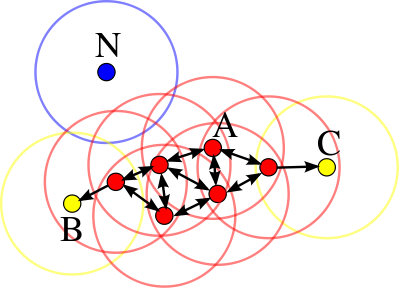
\includegraphics[height=130px]{img/dbscan.png}\end{center}
\begin{itemize}
    \item minPts = 4.
    \item Красные точки -- основные точки. Каждая достижима из каждой
    \item Жёлтые точки не основные, но они достижимы из всех основных. Вместе с красными образуют кластер.
    \item Синяя точка и не основная, и не достижима прямо. Это выброс.
\end{itemize}
Хорошая анимированная визуалиция \href{https://www.naftaliharris.com/blog/visualizing-dbscan-clustering/}{тут}.
\end{frame}

\begin{frame}{Плюсы, минусы, подводные камни}
\begin{itemize}
    \item Умеет находить кластеры любой формы (а не только шарообразные кластеры).
    \item Не нужно знать число кластеров. Хотя надо подбирать параметры minPts и $\varepsilon$.
    \item Всё-таки нужно вводить расстояние между точками (для определения $\varepsilon$-окрестности).
    \item Устойчив к выбросам.
    \item Неоднозначность кластеризации. Особенно по отношению к граничным точкам.
    \item Плохо находит кластеры с большой разницей в плотности.
    \item Средняя сложность $O(N \log N)$. Но это если реализовывать по-умному.
\end{itemize}
    
\end{frame}

\begin{frame}[allowframebreaks]
    \frametitle{Литература}
    \bibliographystyle{unsrt}
    \nocite{esl}
    \nocite{dbscan_wiki}
    \nocite{dbscan_habr}
    \nocite{dbscan_visualization}
    \bibliography{references.bib}
\end{frame}

\end{document}